\graphicspath{{./sixth/img}}

\section*{\LARGE{Введение}}
\addcontentsline{toc}{section}{Введение}
\textbf{Цель}: научиться работать с ресурсами в Android Studio.\par
Ресурс в приложении Android представляет собой файл, например, файл
разметки интерфейса или некоторое значение, например, простую строку. То
есть ресурсы представляют собой и файлы разметки, и отдельные строки, и
звуковые файлы, файлы изображений и т.д. Все ресурсы находятся в проекте
в каталоге res. Для различных типов ресурсов, определенных в проекте, в
каталоге res создаются подкаталоги. Поддерживаемые подкаталоги:

\begin{itemize}
	\item animator/: xml-файлы, определяющие анимацию свойств;
	\item anim/: xml-файлы, определяющие tween-анимацию;
	\item color/: xml-файлы, определяющие список цветов;
	\item drawable/: Графические файлы (.png, .jpg, .gif);
	\item mipmap/: Графические файлы, используемые для иконок приложения;
		под различные разрешения экранов;
	\item layout/: xml-файлы, определяющие пользовательский интерфейс
		приложения;
	\item menu/: xml-файлы, определяющие меню приложения;
	\item raw/: различные файлы, которые сохраняются в исходном виде;
	\item values/: xml-файлы, которые содержат различные используемые в
		приложении значения, например, ресурсы строк;
	\item xml/: Произвольные xml-файлы;
	\item font/: файлы с определениями шрифтом и расширениями .ttf, .otf или
		.ttc, либо файлы XML, который содержат элемент <font-family>.
\end{itemize}

Существует два способа доступа к ресурсам: в файле исходного кода и в
файле xml.
Ссылка на ресурсы в коде
Тип ресурса в данной записи ссылается на одно из пространств (вложенных
классов), определенных в файле R.java, которые имеют соответствующие им
типы в xml:

\begin{itemize}
	\item R.drawable (ему соответствует тип в xml drawable);
	\item R.id (id);
	\item R.layout (layout);
	\item R.string (string);
	\item R.attr (attr);
	\item R.plural (plurals);
	\item R.array (string-array).
\end{itemize}

Нередко возникает необходимость ссылаться на ресурс в файле xml,
например, в файле, который определяет визуальный интерфейс, к примеру, в
activity\_main.xml. Ссылки на ресурсы в файлах xml имеют следующую
формализованную форму: \verb|@[имя_пакета:]тип_ресурса/имя_ресурса|. Где:
\begin{itemize}
	\item имя\_пакета представляет имя пакета, в котором ресурс находится
		(указывать необязательно, если ресурс находится в том же пакете);
	\item тип\_ресурса представляет подкласс, определенный в классе R для
		типа ресурса;
	\item имя\_ресурса имя файла ресурса без расширения или значение
		атрибута android:name в XML-элементе (для простых значений).
\end{itemize}

\clearpage

\section*{\LARGE{Выполнение практической работы}}
\addcontentsline{toc}{section}{Выполнение практической работы}

\section{Ресурсы строк}
Ресурсы строк --- один из важных компонентов приложения. Мы используем
их при выведении названия приложения, различного текста, например, текста
кнопок и т.д.\par
XML-файлы, представляющие собой ресурсы строк, находятся в проекте в
каталоге res/values. По умолчанию ресурсы строк находятся в файле strings.xml,
который может выглядеть следующим образом.\par
Пример использования ресурса проиллюстрирован на
рисунках~\ref{fig:xml:string}\,-\,\ref{fig:java:string}.

\begin{image}
	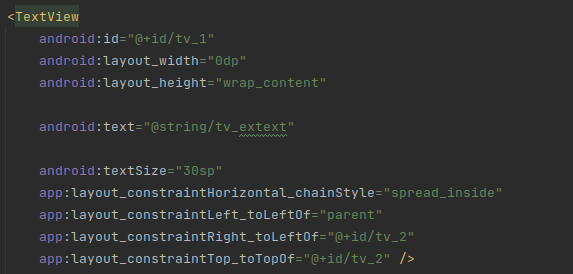
\includegraphics[width=0.8\textwidth]{Screenshot from 2023-03-28 15-20-22.png}
	\caption{Использование ресурсов строк в XML}
	\label{fig:xml:string}
\end{image}

\begin{image}
	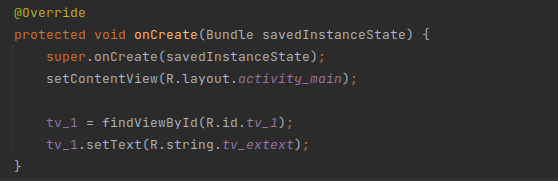
\includegraphics[width=0.8\textwidth]{Screenshot from 2023-03-28 15-30-24.png}
	\caption{Использование ресурсов строк в Java коде}
	\label{fig:java:string}
\end{image}

\section{Форматирование строк}
Android позволяет применять к ресурсам строк форматирование. Пример
показан на рисунке~\ref{fig:format:string}.

\begin{image}
	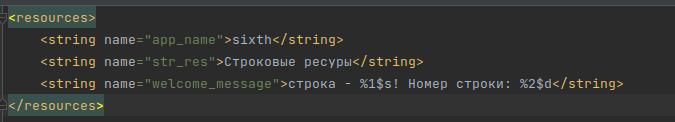
\includegraphics[width=0.8\textwidth]{Screenshot from 2023-03-28 15-40-34.png}
	\caption{Форматная строка в каталоге ресурсов}
	\label{fig:format:string}
\end{image}

Пример использования форматированной строки проиллюстрирован
на рисунках~\ref{fig:java:format}.
\begin{image}
	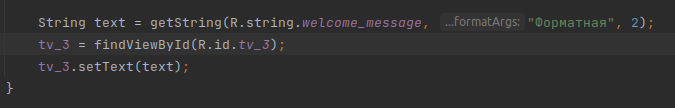
\includegraphics[width=0.8\textwidth]{Screenshot from 2023-03-28 15-44-46.png}
	\caption{Использование форматной строки в Java коде}
	\label{fig:java:format}
\end{image}

\section{}
\section{}
\section{}
\section{}

\clearpage

Создать примеры, реализующие функции ресурсов, изучить виды и работу с
ресурсами. Реализовать два способа доступа к ресурсам: в файле исходного
кода и в файле xml:
1. Реализовать пример использования ресурсов строк
2. Реализовать пример использования форматирование строк.
3. Реализовать пример использования ресурса Plurals
4. Реализовать пример использования ресурса string array
5. Реализовать пример использования ресурса dimension
6. Реализовать пример использования ресурса Color
